\section{Main Result: SSL Gains are Degree-Dependent}
\label{sec:results}

\paragraph{Overall performance.}
Table~\ref{tab:main_gcn} reports AUC and AP for all methods with the GCN backbone. Tables for SAGE and GAT are in the appendix (Tables~\ref{tab:main_sage},~\ref{tab:main_gat}). CL-based methods consistently outperform the supervised baseline across all metrics, with GlobalCL improving overall AUC by 2--6\%. However, these aggregate numbers conceal a strong structural pattern.

\begin{table*}[t]
\centering
\small
\caption{LP performance (mean $\pm$ std, 5 seeds) with GCN backbone. Best cold AUC per dataset in \textbf{bold}. CL methods dominate on cold edges, with gains consistent across AUC and AP.}
\label{tab:main_gcn}
\begin{tabular}{l cccc cccc}
\toprule
& \multicolumn{4}{c}{Cora} & \multicolumn{4}{c}{CiteSeer} \\
\cmidrule(lr){2-5} \cmidrule(lr){6-9}
Method & AUC & AP & Cold AUC & Cold AP & AUC & AP & Cold AUC & Cold AP \\
\midrule
Vanilla & .900 & .899 & .843 & .708 & .864 & .869 & .782 & .672 \\
Reweight & .888 & .892 & .820 & .706 & .888 & .899 & .811 & .725 \\
FocalLoss & .895 & .894 & .843 & .715 & .866 & .871 & .793 & .708 \\
NodeDup & .893 & .897 & .829 & .700 & .890 & .895 & .818 & .722 \\
GlobalCL & .922 & .920 & .884 & .791 & .926 & .931 & .883 & .831 \\
DegGatedCL & .920 & .918 & .885 & .792 & .922 & .924 & .882 & .828 \\
RandomCL & .924 & .923 & \textbf{.889} & \textbf{.801} & .925 & .930 & \textbf{.884} & \textbf{.833} \\
UncertCL & .916 & .918 & .879 & .797 & .915 & .922 & .870 & .822 \\
\midrule
& \multicolumn{4}{c}{PubMed} & \multicolumn{4}{c}{CS} \\
\cmidrule(lr){2-5} \cmidrule(lr){6-9}
Vanilla & .926 & .930 & .898 & .824 & .895 & .890 & .749 & .328 \\
Reweight & .945 & .948 & .924 & .871 & .948 & .945 & .880 & .592 \\
FocalLoss & .923 & .926 & .902 & .828 & .950 & .947 & .894 & .603 \\
NodeDup & .917 & .912 & .898 & .784 & .937 & .933 & .843 & .490 \\
GlobalCL & .949 & .946 & \textbf{.945} & \textbf{.890} & .954 & .952 & .911 & .672 \\
DegGatedCL & .954 & .955 & .938 & .885 & .952 & .948 & .922 & \textbf{.704} \\
RandomCL & \textbf{.956} & \textbf{.956} & .946 & .896 & \textbf{.955} & \textbf{.952} & .908 & .663 \\
UncertCL & .944 & .941 & .940 & .880 & .953 & .950 & .899 & .637 \\
\bottomrule
\end{tabular}
\end{table*}

\paragraph{Degree-stratified gains.}
Figure~\ref{fig:teaser} shows the AUC improvement from GlobalCL over the Vanilla baseline, stratified by min-endpoint training-graph degree. The pattern is striking: on CS, edges with degree 2--4 gain +13.6\%, while edges with degree 20--50 gain only +3.3\%. This monotonic decrease holds across all datasets (Figure~\ref{fig:heatmap}), with the lowest-degree bin consistently showing the largest improvement. We verified this is not purely a headroom artifact: the correlation between degree and SSL gain remains negative (Spearman $\rho < -0.8$ on CS and PubMed) even when controlling for baseline AUC level. All CL vs.\ Vanilla cold-edge AUC differences are significant at $p < 0.05$ (paired $t$-test across seeds).

\begin{figure}[t]
    \centering
    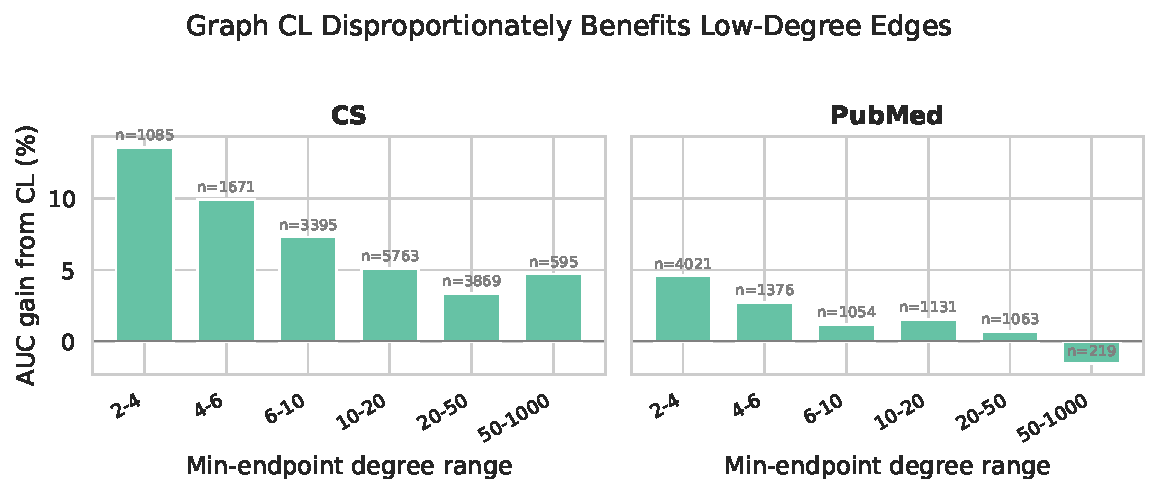
\includegraphics[width=\linewidth]{figures/fig1_teaser.pdf}
    \caption{CL improvement over supervised baseline by degree bin. Gains are monotonically decreasing with degree, with tail edges benefiting up to $4\times$ more than head edges.}
    \label{fig:teaser}
\end{figure}

\begin{figure}[t]
    \centering
    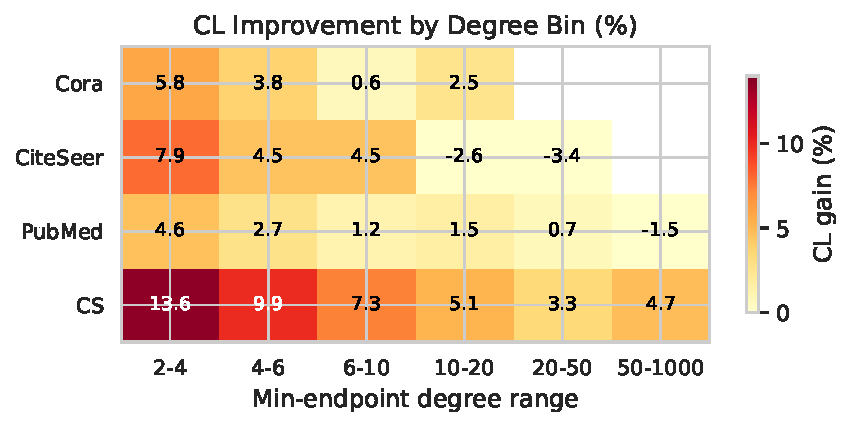
\includegraphics[width=0.9\linewidth]{figures/fig2_heatmap.pdf}
    \caption{CL gain (\%) across datasets and degree bins. The pattern is consistent: low-degree bins always show the largest improvement.}
    \label{fig:heatmap}
\end{figure}

\paragraph{Robustness across backbones and metrics.}
The degree-dependent gain pattern holds across all three backbones (GCN, SAGE, GAT). On GAT---which already achieves higher baseline performance via attention---CL still provides +6\% cold AUC on Cora and +12\% cold AP on CS. The pattern is consistent across AUC, AP, and Hits@20: for every dataset-backbone pair, the cold-edge metric improvement from CL exceeds the warm-edge improvement.

\paragraph{OGB-scale validation.}
On ogbl-collab (235K nodes), self-supervision improves cold-edge AUC from 70.1\% (Vanilla) to 78.9\% (AugOnly) and 78.3\% (GlobalCL), confirming the tail benefit at OGB scale.
